
\begin{figure}
\begin{subfigure}[b]{0.5\textwidth}
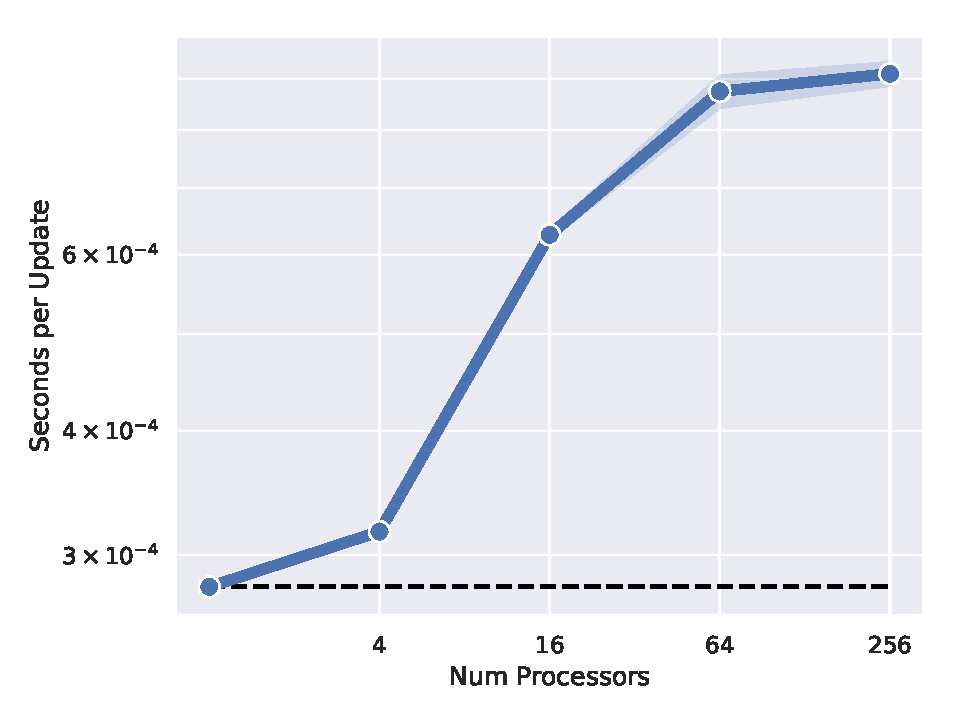
\includegraphics[width=\textwidth]{img/MPIWeak}
\caption{
MPI implementation
}
\label{fig:mpi_weak}
\end{subfigure}
\begin{subfigure}[b]{0.5\textwidth}
  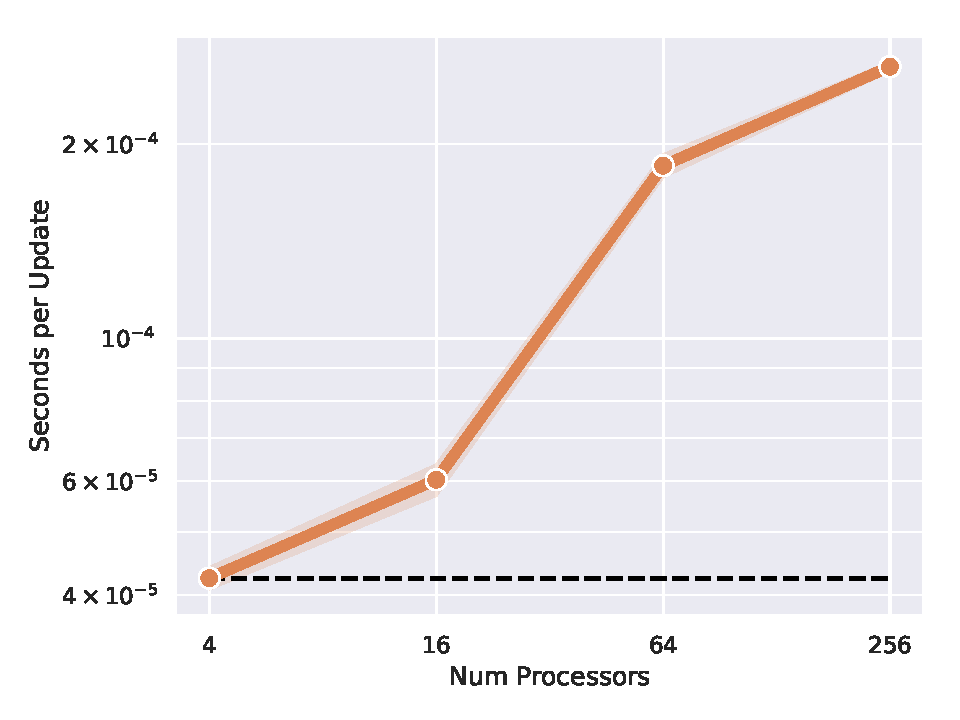
\includegraphics[width=\textwidth]{img/CharmWeak}
\caption{
Charm++ implementation
}
\label{fig:charm_weak}
\end{subfigure}
\caption{
Weak scaling analysis (time to solution versus parallelism with problem size proportional to parallelism) for MPI (\subref{fig:mpi_weak}) and Charm++ (\subref{fig:charm_weak}) implementations.
Dashed line indicates the ideal scaling relationship.
Shaded area represents standard deviation of five replications for each observation.
A problem size of 262,144 grid tiles per CPU was used for the MPI implementation and 1 grid tile per CPU was used for the Charm++ implementation.
}
\label{fig:weak}
\end{figure}
